\section{Software Design}\label{sec:design}
\phantomsection

\subsection{UML Modeling}
The following chapter presents the system modeled in UML language. It contains the main diagrams that are necessary to document and understand the structure and behavior of the system. Before starting any real work, it is essential to define use case diagrams. 

Figure \ref{fig:umlusecase} contains the use case diagram related to the end-user application. This is a high level overview of main features available to users. Respectively, users will be able to access settings, statistics and sleep screen. In settings the user is given the option to set regular sleep time, which includes setting up the start, end of sleep and the days of the week when the user wishes to make the recording. The results of the recording are shown in statistics, which can be erased. Most important screen is the so-called "sleep" screen, where from the recording is being started and ended.

\begin{figure}[!ht]
\centering
  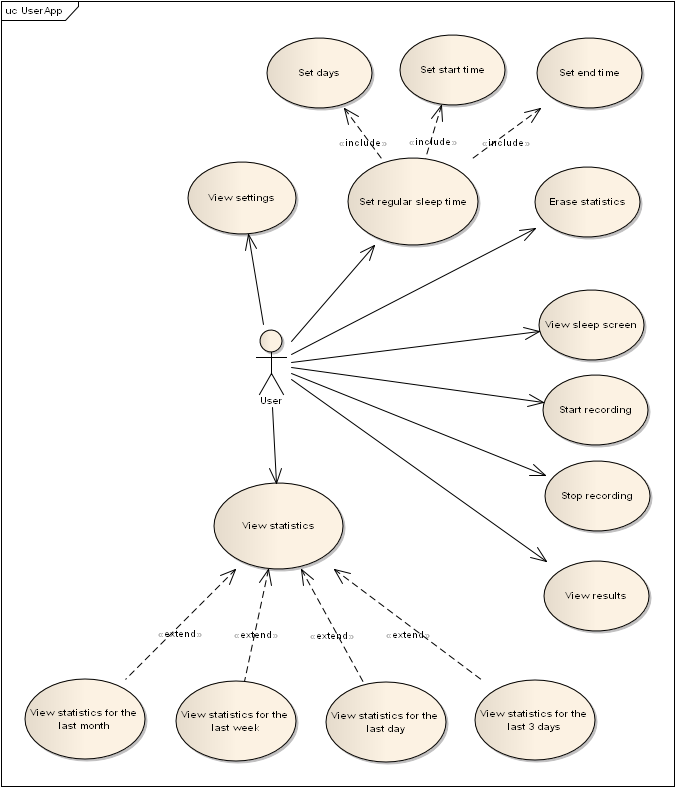
\includegraphics[width=13cm]{uml_usecase.png}
\caption{User application use case diagram}
\label{fig:umlusecase}
\end{figure}

To get a better idea of how the system works, several sequence diagrams are developed. 

\begin{figure}[!ht]
\centering
  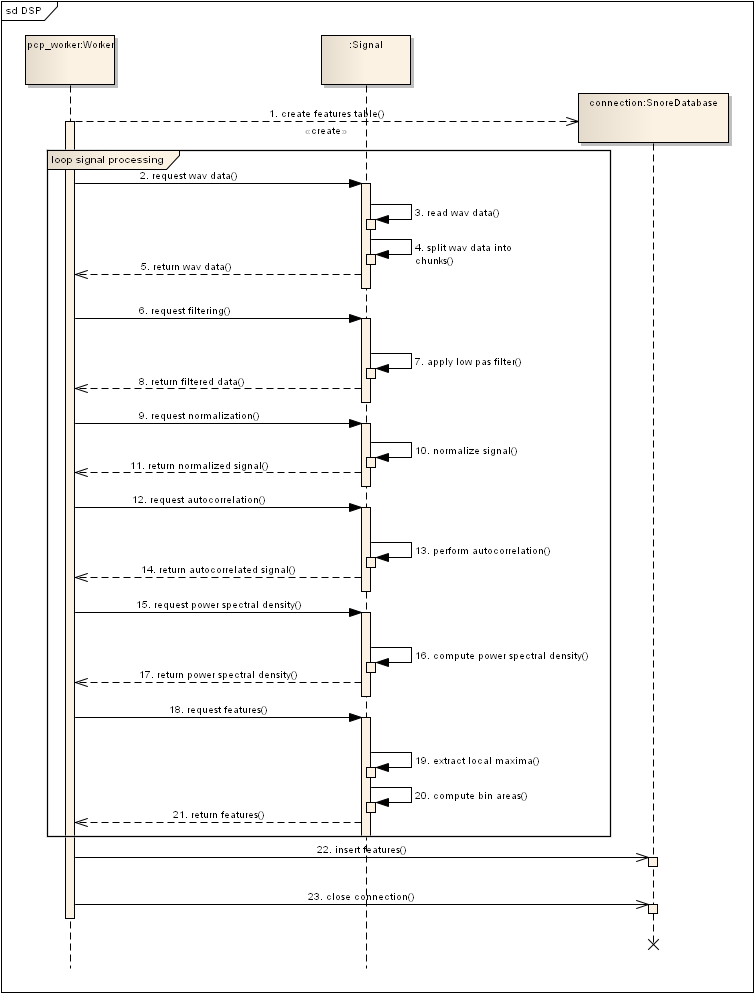
\includegraphics[width=15cm]{uml_dsp.png}
\caption{Digital signal processing sequence diagram}
\label{fig:umldsp}
\end{figure}

\begin{figure}[!ht]
\centering
  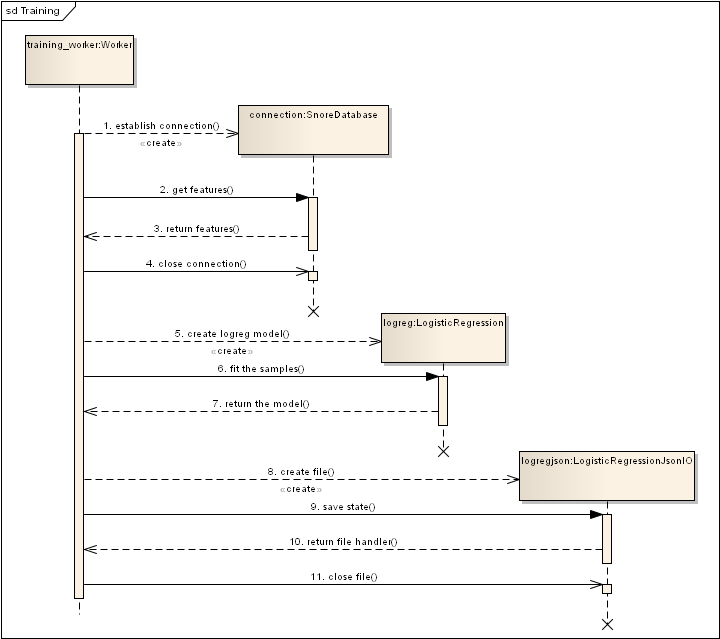
\includegraphics[width=15cm]{uml_training.png}
\caption{Training model sequence diagram}
\label{fig:umltraining}
\end{figure}

\begin{figure}[!ht]
\centering
  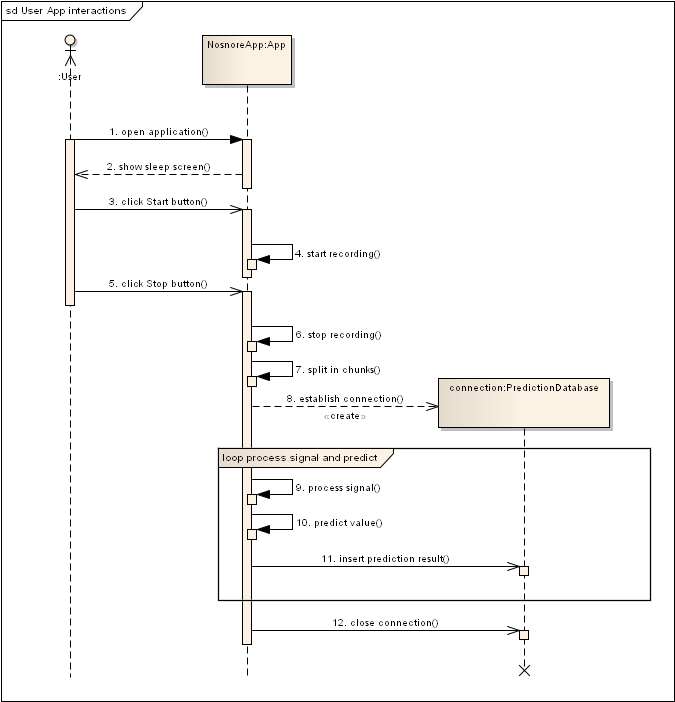
\includegraphics[width=15cm]{uml_userapp_interactions.png}
\caption{User application interactions sequence diagram}
\label{fig:umluserapp}
\end{figure}

\begin{figure}[!ht]
\centering
  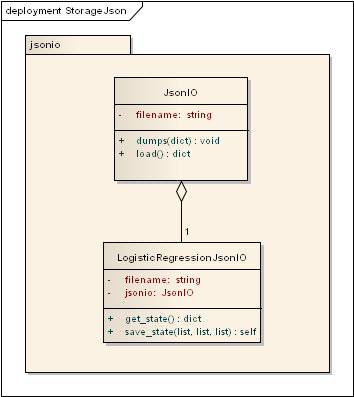
\includegraphics[width=10cm]{uml_class_json.png}
\caption{Json storage class diagram}
\label{fig:umljson}
\end{figure}

\begin{figure}[!ht]
\centering
  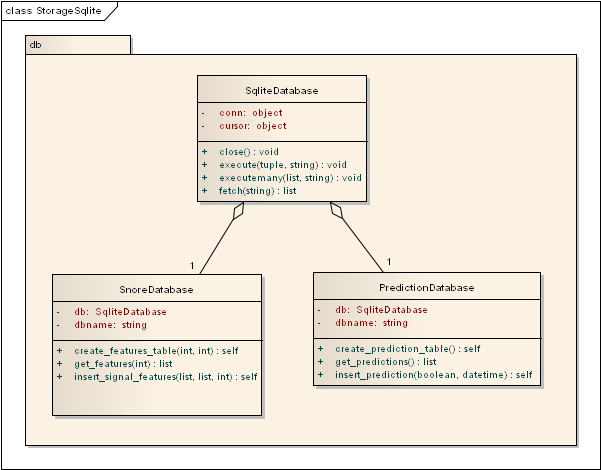
\includegraphics[width=13cm]{uml_class_sqlite.png}
\caption{Sqlite database storage class diagram}
\label{fig:umlsqlite}
\end{figure}

\begin{figure}[!ht]
\centering
  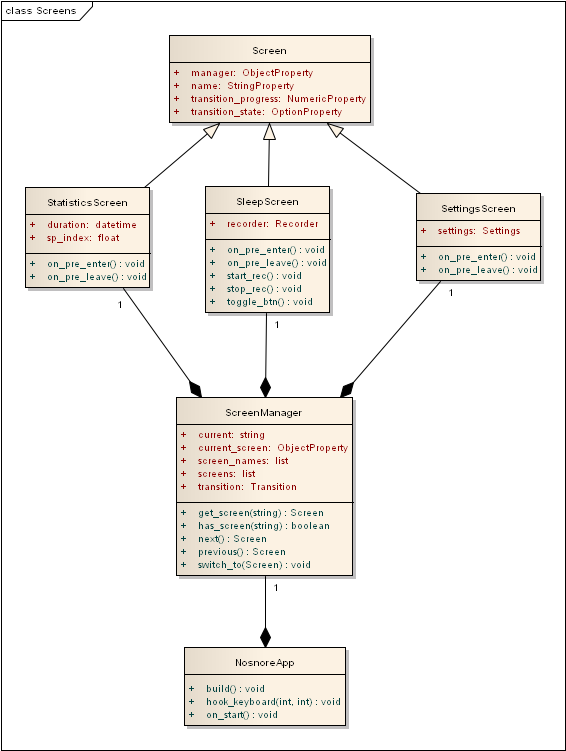
\includegraphics[width=13cm]{uml_class_screens.png}
\caption{Application screens class diagram}
\label{fig:umlscreens}
\end{figure}

\begin{figure}[!ht]
\centering
  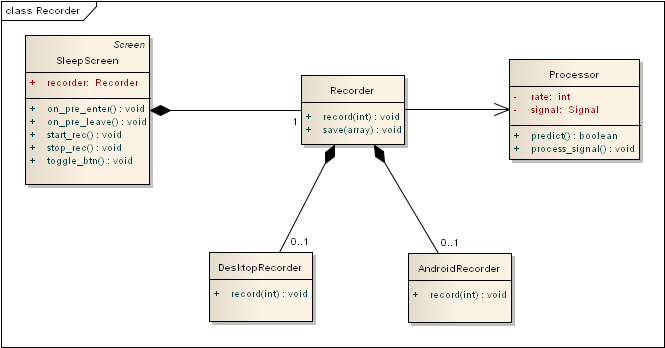
\includegraphics[width=15cm]{uml_class_recorder.png}
\caption{Recorder class diagram}
\label{fig:umlrecorder}
\end{figure}

\begin{figure}[!ht]
\centering
  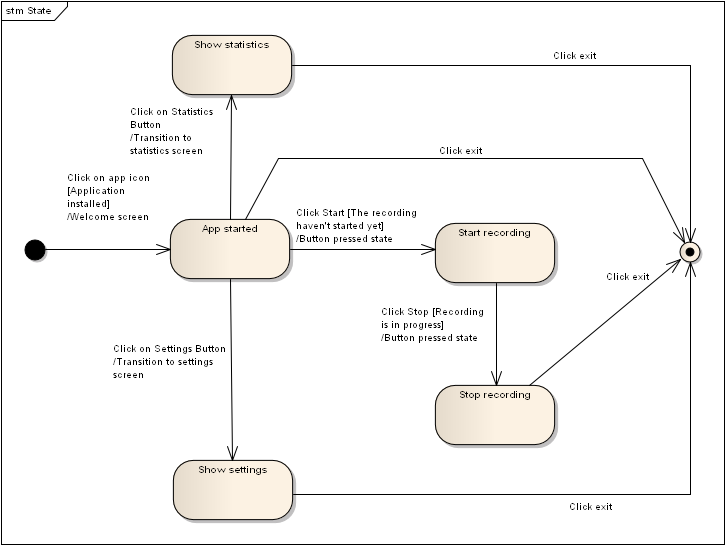
\includegraphics[width=15cm]{uml_state.png}
\caption{App navigation state diagram}
\label{fig:umlstate}
\end{figure}

\begin{figure}[!ht]
\centering
  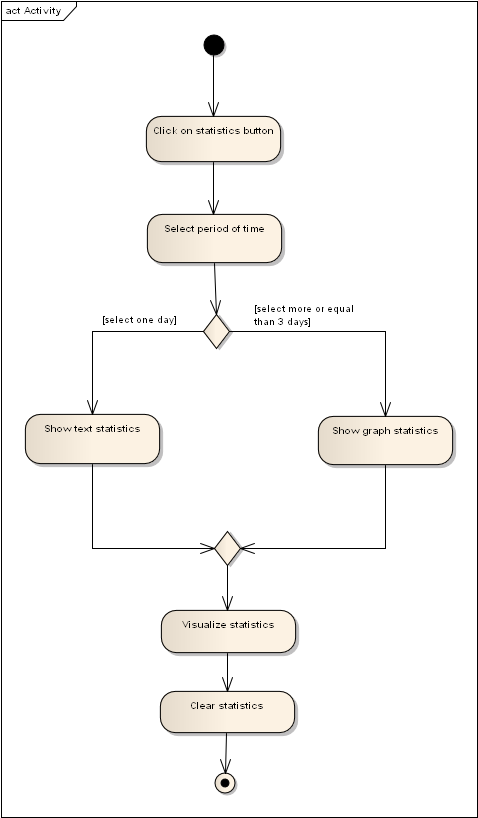
\includegraphics[width=10cm]{uml_activity.png}
\caption{Statistics activity diagram}
\label{fig:umlactivity}
\end{figure}

\begin{figure}[!ht]
\centering
  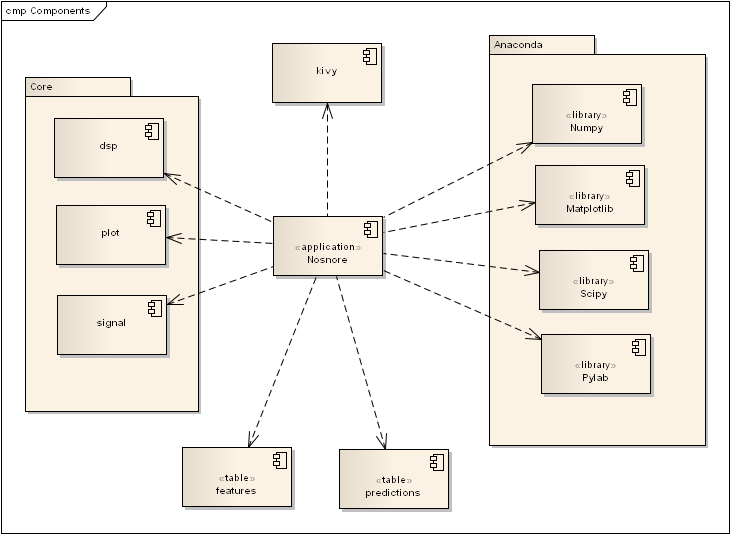
\includegraphics[width=15cm]{uml_components.png}
\caption{Application component diagram}
\label{fig:umlcomponents}
\end{figure}

\clearpage
